%------------------------------------%
%----- 4_Versuchsergebnisse.tex -----%
%------------------------------------%
%------------------------------------%
%
\subsection{Messdaten}
\label{subsec:4_Daten}
%
Die Messergebnisse sind in Tab. \ref{tab:4_Messdaten} dargestellt\footnote{Alle Werte aufgenommen bzw. berechnet von \autorA}.
%
\begin{table}[H]
  \small
  \centering
	\caption{Messergebnisse}
	\label{tab:4_Messdaten}
	\begin{tabular}{rrrrrr}
	  \toprule
		%
	  \multicolumn{1}{c}{Einstellwerte} &
		\multicolumn{3}{c}{Messwerte} &
		\multicolumn{2}{c}{Berechnete Werte} \\
		\cmidrule(lr{1mm}){1-1}\cmidrule(lr{1mm}){2-4}\cmidrule(lr{1mm}){5-6}
		%
		$f_\mathrm{E}$ in \si{\hertz} &
			$U_\mathrm{E,pp}$ in \si{\volt} &
    		$U_\mathrm{A,pp}$ in \si{\volt} &
    		$\Delta t$ in \si{\micro\second} &
    			$|\underline{H}|_\mathrm{dB}$ in \si{\decibel} &
				$\mathrm{arg}(\underline{H})$ in \si{\degree}\\
		\midrule
		%
    \input{src/4_Messdaten.txt}
    %
		\bottomrule
	\end{tabular}
\end{table}
%
Die Formeln dafür sind
\[m|\underline{H}|_{dB}=20\log(\frac{U_{A,pp}}{U_{E,pp}})\]
\[{\varphi}_{\underline H}=360^\circ \cdot arg(\underline{H})=360^\circ \cdot f_E \cdot \Delta t \]
%
%
\newpage
\subsection{Ergebnisplots}
\label{subsec:4_Plots}
%
%------------------------------%
%----- Beginn eures Teils -----%
%------------------------------%
%
\begin{figure}[H]
	\centering
	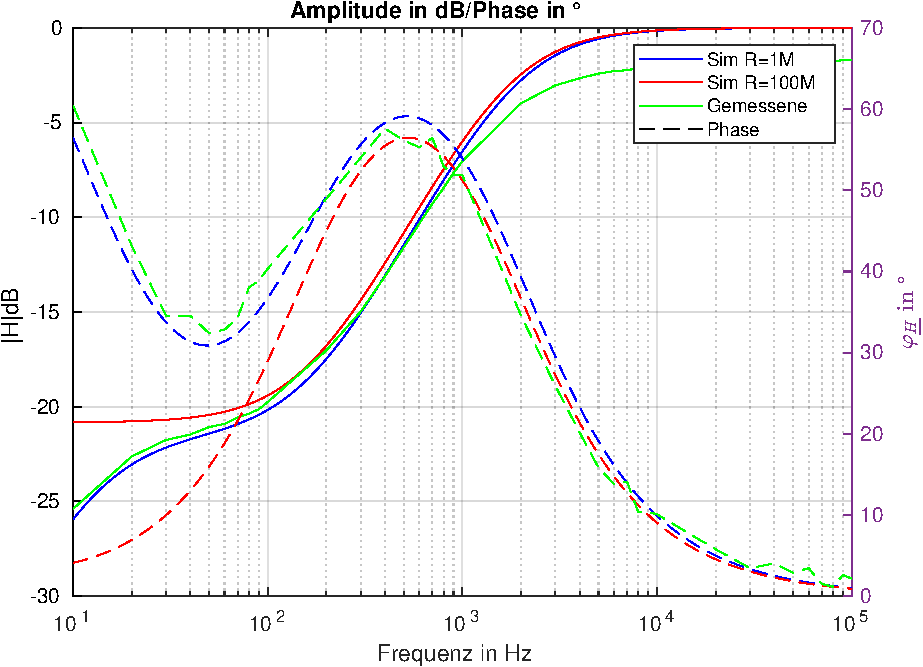
\includegraphics[scale=.8]{src/labor5.pdf}
	\caption{Bode Plot für verschiedene Werte von $R$}
	\label{fig:Bode Plot Simulation}
  \end{figure}
%
%
%
$R_{mess}$ wirkung ist am kleinsten wenn die Frequenz höher als ungefähr 100Hz, aber wenn die Frequenz sehr gering ist, Rmess hat ein sehr großere Wirkung, am kleine Frequenzen je geringer die Widerstand desto großere Amplitude erhält man. Der Grund dafür ist dass, der Messwiderstand mit C1 einen Hochpass bildet. Dadurch wird bei kleinen Frequenzen die Amplitude gedämpft und die Phase angehoben. Je größer der Messwiderstand ist, desto geringer ist der Einfluss.


\begin{flushright}
  \textit{\autorA}
\end{flushright}
%
%------------------------------%
%------ Ende eures Teils ------%
%------------------------------%
%
%
%